Where as memory access optimization can be related to warps, thread divergence is purely related to how threads are executed within a warps. As described in \cref{sec-hw-warps-threads} a warp is a Single Instruction Multiple Threads unit, which can only run a single instruction set at a given time on all threads, which means every time a branching is encounters, some threads might stale while others instruction set is being executed. And example of branch divergence could be based on an simple switch case with in a kernel. For branch divergence only the case it self is important which can be seen in listing \ref{lst:branch_div}.\\

\begin{lstlisting}[language=C,caption={Dividing threads into warps, using modulus operator},label=lst:branch_div]
switch(thread_id % 2)
{
	case 0:
		sdata[id]--;
	case 1:
		sdata[id]++;
}
\end{lstlisting} 

So the kernel in listing \ref{lst:branch_div} would be a simple program kernel which access some shared memory, and if the index of the shared memory is even, its decremented, if it is odd its incremented. To fully understand how this example would be influence by branch divergence, it is important to understand how the thread IDs are assigned, as in this, and most other cases, it is the ID which would be used to determine branching. As described in \cref{sec-pm-threads} threads receive both a X, Y and Z id with in their block, and their block receives a X, Y and Z index as well. From these a global id can be constructed which is normally what is used when writing CUDA programs. When threads are assigned to Warps, this happens by first assigning along the X IDs, then the Y IDs and last the Z IDs. Thereby if a block is created with X dimension of 32 and a Y dimension of 32, as Warps contain 32 threads we will have that all threads with in the Warp has the same Y ID and X ID ranging from 0 to 31. A visualization of this can be seen in \cref{fig:id_warp}.\\

\begin{figure}[ht]
	\centering
	\fbox{
		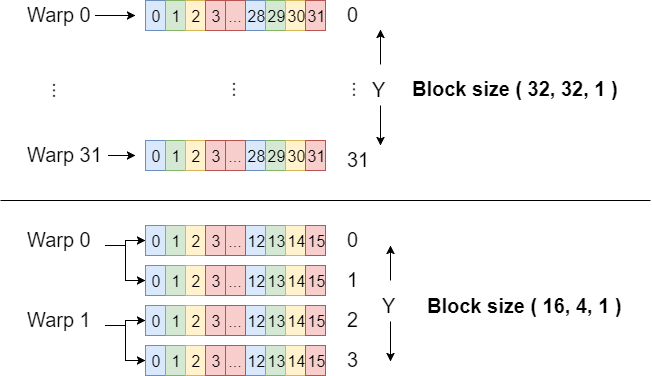
\includegraphics[width=0.9\textwidth]{figs/opti/ID_warp.png}
	}
	\caption{Threads ID's inclusion in Warps.}
	\label{fig:id_warp}
\end{figure}

Based on the before mentioned kernel being executed with a block size of (32, 32 1), and using the knowledge of how thread ID's are assigned, it can then be determined that every second thread within a Warp will take the first case, and every other will take the second case. Had this been a computation which far out weighted that of the switch case and calculating the global index, the execution time would be approaching two time that which would be expected if there had been no such thing as Warps.\\

Therefore, while thread divergence may not always be a huge factor when it come to slow downs, it is worth noting that thread divergence within Warps clearly effect the execution time of a kernel. Which means that there are cases where i might be worth optimizing threat divergence. The approach here is to arrange the branches or data different, such that more threats within a Warp will take the same route through the code of the kernel. For the code listed in listing \ref{lst:branch_div} this could have been achieved by having another data arrangement and then changing the code to what can be seen in listing \ref{lst:branch_div2}.

\begin{lstlisting}[language=C,caption={Creating a better arrangement of threads to allign with warps},label=lst:branch_div2]
switch(thread_id / 32)
{
	case 0:
		sdata[id]--;
	case 1:
		sdata[id]++;
}
\end{lstlisting} 

And while it may not be possible for all code to do such a rearrangement, similar optimization might be worth considering if optimizing performance critical applications with a lot of branching.